\documentclass[a4paper,10pt, margin=0.75in]{article}
\usepackage[utf8]{inputenc}
\usepackage{graphicx}

\usepackage[square,numbers,amsmath]{natbib}
\bibliographystyle{unsrtnat}
\usepackage{amsfonts,amssymb}
\usepackage{mathtools}

\title{Statistical Identification of Multiple Bugs Through Implicit Biclustering}
\author{Jaivardhan Kapoor, Shivansh Rai}

\begin{document}

\maketitle

\begin{abstract}
    The problem of bug localization and triage is usually accompanied by a similar challenge of understanding the causal factors behind each failure, as there can be multiple bugs. In this term paper, we attempt to look at a review of prevalant bug localization methods. We also look at certain approaches of multiple simultaneous bug localization, and focus particularly on a specific approach which uses statistical methods to implicitly bicluster runs and predicates to identify multiple bug clusters. We test the approach on small programs to gauge its efficacy and comment on the results obtained.
\end{abstract}

\section{Introduction}
Automated debugging of software is a very active research area. One factor that drives this activity is that the mass of written code is continuously increasing at an ever increasing rate, which creates more bugs and more problems to solve. another factor behind this is that major software repositories of large communities and corporations have very large codebases. These codebases obviously bugs interspersed in them, and debugging on such a large codebase may be very taxing if done manually using conventional tools. Also, such large codebases regularly get feedback and reports from users and developers alike, which result in the gathering of large amount of data and thus a better chance of bug localization through data analysis, which may easily be done better using a computer.\\
Once the possible locations of a bug are identified using a localization tool, a human expert(in this case, a tester or developer) identifies the possible candidates and rules out if the candidates are false positives or real big causes/locations. This feedback by the developer may be then used again by the tool to further improve its candidate ranking and detection algorithm using statistical or machine learning techniques. We will, in this paper, look at some seminal bug localization methods that leverage the large body of information gathered from multiple runs of a program, and use statistical methods to provide locations and predictors for bugs in both single as well as multiple bug setting.\\
The specific case of multiple bug localization is more difficult to analyze and correct than the single bug problem. The reason for this is that multiple bugs may interact within themselves, and these cross interactions may make it difficult to decipher the cause of a failed run. Also, failed runs and cases are not explicitly labeled along with the bug that caused them. This results in the problem being similar to a clustering problem, where we do not know the cluster id's of the runs and also the number of clusters. Here the clusters are analogous to the different bugs present in the program. We will see in this later section that this formulation of the multi-bug problem can be used for developing a biclustering approach to solving the problem.\\
The rest of the article is arranged as follows: Section 2 discusses related work and approaches, and Section 3 presents a multi-bug identification approach using implicit biclustering. We discuss various experiments conducted, along with results obtained and their interpretations, in Section 4 and Section 5 respectively. Section 6 finally concludes the paper.

\section{Related Work}
Statistical debugging usually involves data that is collected throughout the runtime of the program. Examples include truth values and frequencies of certain boolean predicates like \texttt{(f == NULL)}, or memory dumps and execution traces of programs. These are commonly used \textit{spectral methods}, and are used widely with many techniques. Certain approaches also leverage the power of static analysis tools for small parts of the code in which the tool suspects the localized bug lies.\\
There is a lot of literature pertaining to statistical debugging. We will be discussing 2 main papers that contributed greatly to the state-of the-art when they were published, which have already been discussed in class.\\
The first approach\cite{DBLP:conf/pldi/LiblitNZAJ05} uses truth values of predicates in hypothesizing whether a predicate is useful in predicting erroneous behaviour of a program caused by bugs. The paper presents some hypotheses for code behaviour which are obtained by direct observation of the behaviour of programs in real world and distribution and manifestations of bugs in real world codebases. It works on the assumption that predicates which hit their truth value in multiple runs very often are more likely to predict bugs if they hit a false value in a run, and then that predicated is considered as a predictor of a bug for that failed run. This is formulated in the paper as a \textit{weak hypothesis}, which formally states that predicates with more successful runs are more likely to be predictors i they hit false values for less failed runs. Contrary to this, the strong hypothesis stated works on the principle that predicates having many false values are less likely to be predictors of bugs that result in them manifesting false values, and are more likely to be false positives. A direct consequence of these 2 hypotheses is that predictors which are only hitting their false values are extremely unlikely to predict any bugs. The paper then continues to formulate their ranking and predictor identification scheme using various importance scores which also take into account the context of the predictor used through various simple statistical techniques.\\
One clear flaw in this work was that the frequencies of hits of predicates in a single run was not taken into account. This resulted in some of the cases of bug detection being missed. This problem was alleviated in another work\cite{DBLP:conf/sigsoft/LiuYFHM05}. Their tool, called \texttt{SOBER}, uses the number of hits of each of the boolean values of the predicates in each run and uses statistical techniques to measure its effect on the set of failing and successful runs separately. A predicate is considered to be a valid predictor of a certain bug, if its behaviour changes significantly among the set of failing and successful runs respectively. This was better suited to identifying some cases that were not so apparent in the precious work.\\
These approaches made an assumption that the top ranked predicates predicted different bugs, that is, they were disjoint in their prediction of bugs. This may not always be the case, as a failed run may be the result of many bugs happening at once. This problem is alleviated by jointly clustering the runs and predicates such that different 'sub'clusters obtained predict different bugs, These 'sub'clusters may be overlapping or even nested, which accounts for different cases. The following section discusses this approach in detail.

\section{Multiple bug identification through implicit biclustering}
In this section we look at another paper by Liblit, Jordan et al.\cite{DBLP:conf/icml/ZhengJLNA06} which uses a collective voting scheme between runs and predicates and a probabilistic graphical model to infer the qualities of valid predicates.
\subsection{An Approach to Biclustering}
Biclustering is jointly clustering 2 different items or categories into different kinds of clusters that may be overlapping, nested or clustered in a specific way. The following figure represents different types of biclusters that can be formed. We will refer this during our next discussion on the algorithm used.
\begin{figure}[h]
    \centering
    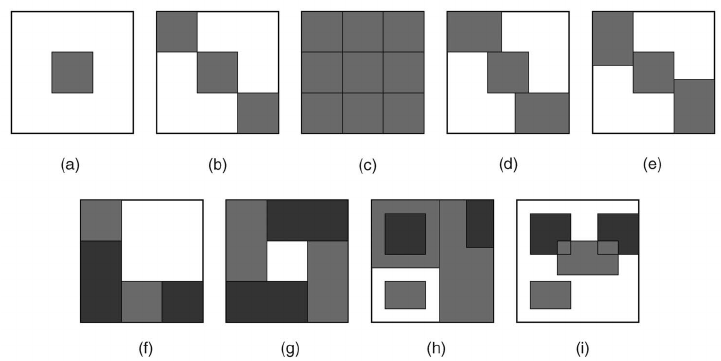
\includegraphics[width=\linewidth]{bivluster.png}
    \caption{Types of biclusters}
\end{figure}

\subsection{Collective Voting Scheme}
The truth probabilities of predicaates in different runs are obtained through instrumentation data. Further, we have knowledge of set of runs failed and succeeded. Let us denote them by $F$ and $S$ respectively. We then operate on the driving principle that the predicate should cluster by the runs and vice-versa.\\
Each predicate is assigned a quality factor $Q$, which determines its relevance for bug isolation. All attributes related to a predicate are also evaluated for its complement. Thus $Q_i$ and $Q_\overline{i}$ denote the wualities of predicate i and its complement respectively. Similarly, the vote or weight given by run $j$ to predicate $i$ is denoted by $R_{ij}$, and its vote to the predicate's complement as $R_{\overline{i}j}$. Similarly, predicate i's contribution to the set of failing runs is defined as $F_i$ and its contribution to the set of successful runs as $S_i$, with repspective notations applying for the complement's contributions to the same. $A_{ij}$ is the truth probability of predicate i in run j.\\
The algorithm is an iterative one, which runs till the convergence of the rankings of predicates by their quality. The update equations for the attributes of the predicates and runs are as follows:
$$
\begin{aligned}
    Q_i&=\frac{F_i}{S_i}\frac{S_\overline{i}}{F_\overline{i}} & Q_\overline{i}&=\frac{S_i}{F_i}\frac{F_\overline{i}}{S_\overline{i}}\\
    F_i&=\sum_{j\in F}A_{ij}\frac{R_{ij}}{\sum_{k\in pred}R_{kj}} & F_\overline{i}&=\sum_{j\in F}A_{\overline{i}j}\frac{R_{\overline{i}j}}{\sum_{k\in pred}R_{\overline{k}j}}\\
    S_i&=\sum_{j\in S}A_{ij}\frac{R_{ij}}{\sum_{k\in pred}R_{kj}} & S_\overline{i}&=\sum_{j\in S}A_{\overline{i}j}\frac{R_{\overline{i}j}}{\sum_{k\in pred}R_{\overline{k}j}}\\
    R_{ij}&=\begin{cases}
        A_{ij}\cdot Q_i & \text{if } j\in F,\\
        A_{ij}/Q_i & \text{if } j\in S
    \end{cases} & R_{\overline{i}j}&=\begin{cases}
        A_{\overline{i}j}\cdot Q_\overline{i} & \text{if } j\in F,\\
        A_{\overline{i}j}/Q_\overline{i} & \text{if } j\in S
    \end{cases}\\
\end{aligned}
$$
These 4 equations implicitly bicluster the predicate-runs space into (ideally) the (b) part of the above figure. This ensures the biclusters obtained are somewhat disjoint and able to properly predict different causes of biclustering, which in this case are the multiple bugs in the program.
\section{Experiments}
\subsection{Procedure}
% \subsubsection{Generating predicates from a program runtime}
% The predicates being used in the implementation are combinatoric relations between all the variables in a program, resulting in \binom{N}{K} predicates.
% The daikon frontend is used for collecting states of the variables inside all the functions in a program. These states are then parsed, and a python script containing the \binom{N}{K} predicates is generated. Corresponding to the obtained values of the variables, the frequency of each predicate is incremented. Hence, at the end of a single execution, we have a set of \binom{N}{K} predicates with there corresponding frequency of hits during runtime.
% This procedure is then repeated for multiple inputs.

\subsubsection{Instrumentation for generating predicates}
For the purposes of this project, every if statement in a program is counted as a valid predicate. \\
Rose has been chosen as the instrumentation framework for instrumenting all the if statements in a given input program. For each if statement, it is noted as whether the condition evaluated to true or false. For each predicate, the number of times it was encountered during the execution is also noted. The structure of a predicate is thus a pair of values, where the first value determines how many times the predicate was evaluated to true and the second value determines how many times the predicate was evaluated to false. \\
The total number of collected predicates from both the server and the client were 38.

\subsubsection{Testing framework}
The current framework is tested on a client-server model. In each run, the client requests a file from the FTP server. The success and failure of the run is determined by the availability of the requested file at the server.

\subsubsection{Random bug insertion}
Before the beginning of each execution, a bug is inserted randomly into the client code. The client code already contains bugs which are wrapped around by relevant preprocessor directives. \\
For e.g. a bug numbered n is inside the following preprocessor directive -
\begin{verbatim}
                        #ifdef BUGn
\end{verbatim}
This ensures that every time the preprocessor directive surrounding a certain bug evaluates to true, that bug will be automatically inserted in the client code. \\
To randomly insert bugs, a script is written which generates a random bug number, with which it creates a string which looks as follows -
\begin{verbatim}
                            #define BUGn
\end{verbatim}
This string is then inserted into one of the header files which the client inherits, and then the client code is recompiled, resulting in the insertion of \texttt{BUGn} in it. \\
The above process is repeated for an arbitrary number of bugs.

\subsubsection{Experiment setup}
The experiment is carried out with the client requesting 20 valid and 20 invalid files from the server, resulting in 20 successful and 20 failed runs. For each run the predicate values from both the client and the server are collected. For getting a deterministic failing run, a bug is inserted in the client which clobbers the filename retrieved from the command line argument given to the client binary. Thus the client ends up requesting an invalid file in that run.


\section{Results and Conclusion}
After evaluating the predicates collected from the experiment, predicate number 20 seems to be ranked highest among all the predicates. This predicate is present in the server code and corresponds to the if statement which checks the presence of the file requested by the client. This points out to the fact that the client (user) requested an invalid file, and there can be 2 possible reasons for this -
\begin{itemize}
    \item The user gave an invalid filename as a command line argument while executing the client.
    \item The user gave a valid filename as a command line argument but the client code incorrectly manipulated it, and ended up requesting a different file.
\end{itemize}

The second case is valid for the above experiment, and predicate number 20 implicitly points out to it.

\medskip

\bibliography{sample}

\end{document}
